\documentclass{article}

\usepackage{graphicx}
\usepackage{tikz}
\usepackage{tikzsymbols}
\usetikzlibrary{calc,patterns,shapes.geometric}
\pagestyle{empty}
\usepackage[margin=0pt]{geometry}
\geometry{papersize={14in,12in}}

\def\centerarc[#1](#2)(#3:#4:#5){\draw[#1] ($(#2)+({#5*cos(#3)},{#5*sin(#3)})$) arc (#3:#4:#5);}

\begin{document}
	\begin{figure}
		\centering
		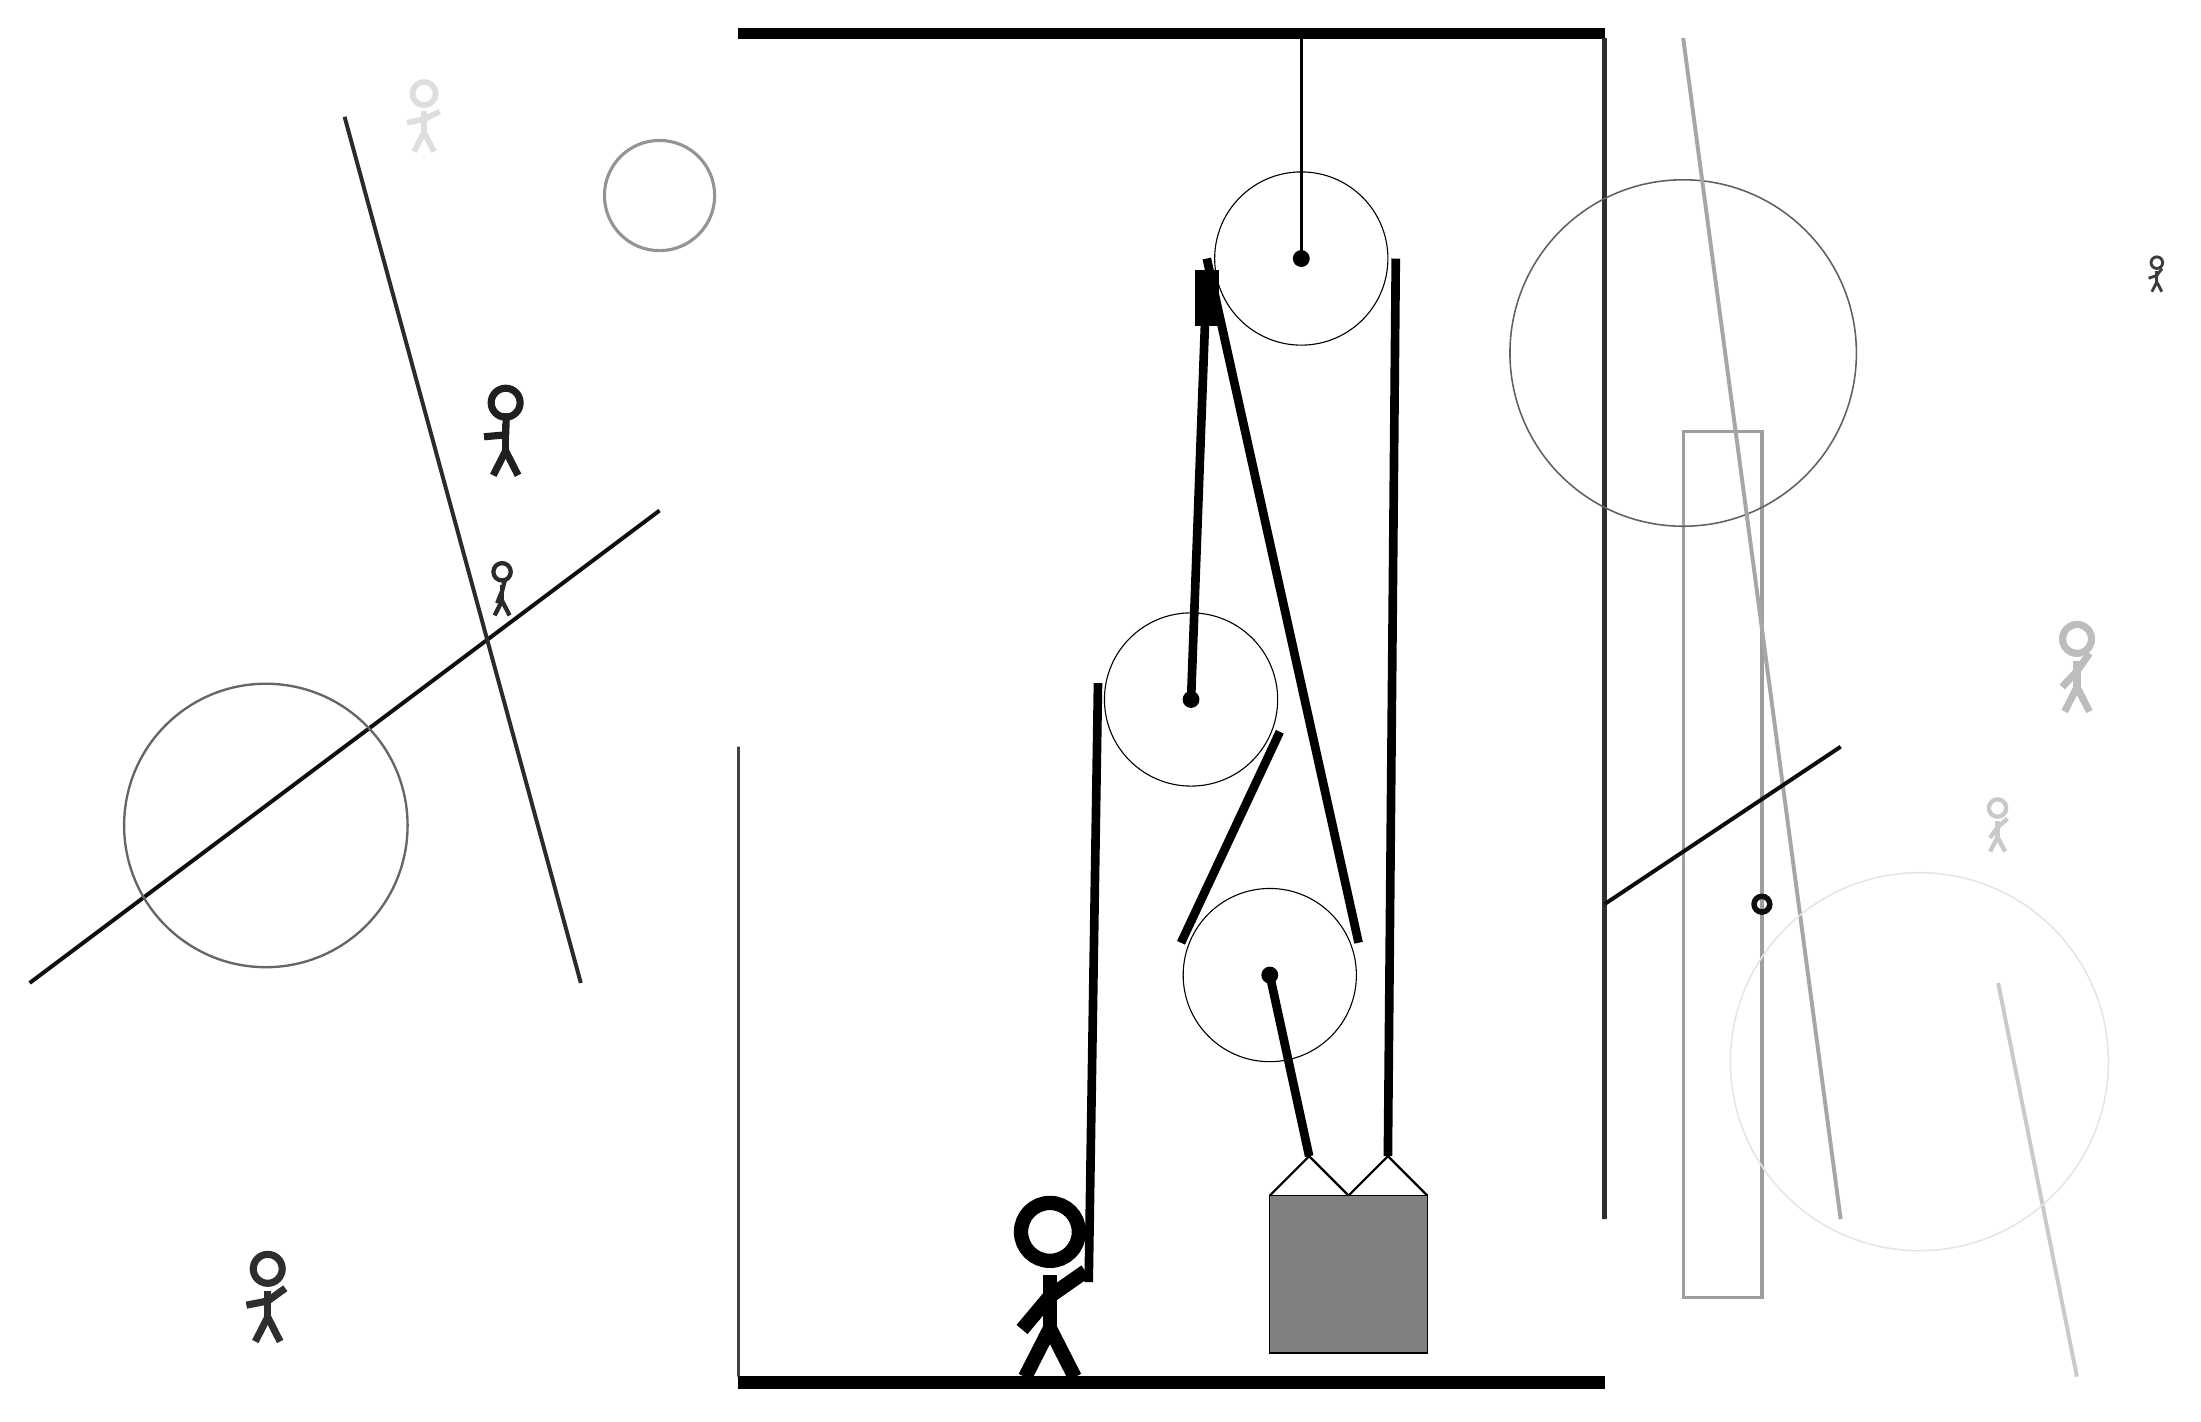
\begin{tikzpicture}
			%%%%% START %%%%%
			
			\draw[fill=black] (-6, 14) rectangle (5, 14.125);
			
			\draw[line width=0.4mm, color=black!38] (6, -2) rectangle (7, 9);
			
			\draw[line width=0.5mm, color=black!94](-7, 8) -- (-15, 2);
			\node[line width=0.6mm, color=black!76] at (12, 11) {\Strichmaxerl[2][18][54]};
			\draw[line width=0.5mm, color=black!21](10, 2) -- (11, -3);
			\draw[line width=0.6mm, color=black!82] (5, -1) rectangle (5, 14);
			
			\draw [line width=0.7mm, color=black!94](7, 3) circle (0.1);
			
			\draw [line width=0.2mm, color=black!62](6, 10) circle (2.2);
			\node[line width=0.6mm, color=black!13] at (-10, 13) {\Strichmaxerl[4][11][26]};
			\node[line width=0.2mm, color=black!88] at (-9, 9) {\Strichmaxerl[5][5][88]};
			\draw[line width=0.5mm, color=black!35](6, 14) -- (8, -1);
			
			\draw[line width=0.5mm, color=black!95](5, 3) -- (8, 5);
			\node[line width=0.7mm, color=black!82] at (-12, -2) {\Strichmaxerl[5][11][36]};
			\draw [line width=0.4mm, color=black!42](-7, 12) circle (0.7);
			
			\node[line width=0.4mm, color=black!26] at (11, 6) {\Strichmaxerl[5][47][55]};
			\draw[line width=0.5mm, color=black!83](-11, 13) -- (-8, 2);
			\draw [line width=0.2mm, color=black!10](9, 1) circle (2.4);
			
			\draw[line width=0.4mm, color=black!74] (-6, -3) rectangle (-6, 5);
			
			\draw [line width=0.3mm, color=black!60](-12, 4) circle (1.8);
			\draw[line width=0.5mm, color=black!38](5, 11) -- (5, 11);
			\node[line width=0.6mm, color=black!83] at (-9, 7) {\Strichmaxerl[3][68][76]};
			\node[line width=0.3mm, color=black!21] at (10, 4) {\Strichmaxerl[3][54][41]};
			
			\draw (-0.25, 5.6) circle (1.1);
			\draw[fill=black] (-0.25, 5.6) circle (0.1);
			
			\draw (0.75, 2.1) circle (1.1);
			\draw[fill=black] (0.75, 2.1) circle (0.1);
			
			\draw (1.15, 11.2) circle (1.1);
			\draw[fill=black] (1.15, 11.2) circle (0.1);
			\draw[very thick] (1.15, 11.2) -- (1.15, 14);
			
			\draw[thick]  (0.75, -0.7) -- (1.25, -0.2) -- (1.75, -0.7) -- (2.25, -0.2) -- (2.75, -0.7);
			\draw[fill=black!50] (0.75, -0.7) rectangle (2.75, -2.7);
			
			\draw[line width=1.1mm] (-0.25, 5.6) -- (-0.05, 11.0);
			\draw[line width=1.1mm, fill=black](-0.15, 10.4) rectangle (0.05, 11.0);
			\draw[line width=1.1mm] (-1.55, -1.8) -- (-1.4318, 5.8083);
			\centerarc[line width=1.1mm](-0.25, 5.6)(-20:170:1.2000000000000002);
			\draw[line width=1.1mm] (0.8776, 5.1896) -- (-0.3776, 2.5104);
			\centerarc[line width=1.1mm](0.75, 2.1)(160:380:1.2000000000000002);
			\draw[line width=1.1mm] (1.8776, 2.5104) -- (-0.05, 11.2);
			\draw[line width=1.1mm](0.75, 2.1) -- (1.25, -0.2);
			\centerarc[line width=1.1mm](1.15, 11.2)(0:180:1.2000000000000002);
			\draw[line width=1.1mm] (2.35, 11.2) -- (2.25, -0.2);
			
			\node at (-2, -1.9) {\Strichmaxerl[10][50][35]};
			
			\draw[fill=black] (-6, -3) rectangle (5, -3.15);
			
			%%%%% END %%%%%
		\end{tikzpicture}
	\end{figure}	
\end{document}